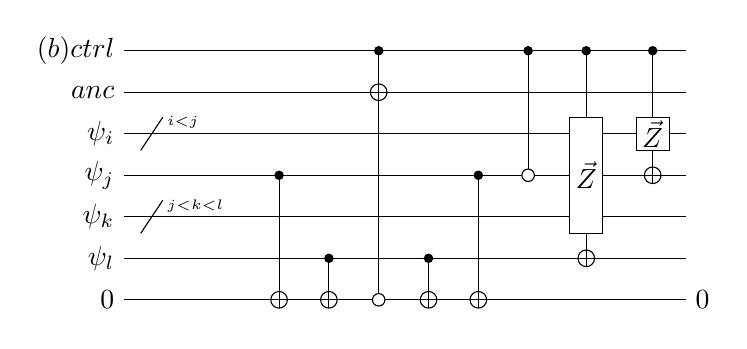
\begin{tikzpicture}[scale=1.000000,x=1pt,y=1pt]
\filldraw[color=white] (0.000000, -7.500000) rectangle (203.000000, 97.500000);
% Drawing wires
% Line 1: c W \text{(b) }ctrl
\draw[color=black] (0.000000,90.000000) -- (203.000000,90.000000);
\draw[color=black] (0.000000,90.000000) node[left] {$\text{(b) }ctrl$};
% Line 2: a W anc
\draw[color=black] (0.000000,75.000000) -- (203.000000,75.000000);
\draw[color=black] (0.000000,75.000000) node[left] {$anc$};
% Line 3: i W \psi_i
\draw[color=black] (0.000000,60.000000) -- (203.000000,60.000000);
\draw[color=black] (0.000000,60.000000) node[left] {$\psi_i$};
% Line 4: j W \psi_j
\draw[color=black] (0.000000,45.000000) -- (203.000000,45.000000);
\draw[color=black] (0.000000,45.000000) node[left] {$\psi_j$};
% Line 5: k W \psi_k
\draw[color=black] (0.000000,30.000000) -- (203.000000,30.000000);
\draw[color=black] (0.000000,30.000000) node[left] {$\psi_k$};
% Line 6: l W \psi_l
\draw[color=black] (0.000000,15.000000) -- (203.000000,15.000000);
\draw[color=black] (0.000000,15.000000) node[left] {$\psi_l$};
% Line 7: c0 W 0 0
\draw[color=black] (0.000000,0.000000) -- (203.000000,0.000000);
\draw[color=black] (0.000000,0.000000) node[left] {$0$};
% Done with wires; drawing gates
% Line 9: i / ^{i<j}
\draw (6.000000, 54.000000) -- (14.000000, 66.000000);
\draw (12.000000, 63.000000) node[right] {$\scriptstyle{^{i<j}}$};
% Line 10: k / ^{j<k<l}
\draw (6.000000, 24.000000) -- (14.000000, 36.000000);
\draw (12.000000, 33.000000) node[right] {$\scriptstyle{^{j<k<l}}$};
% Line 11: c a i j k l c0 LABEL
% Line 12: j +c0
\draw (56.000000,45.000000) -- (56.000000,0.000000);
\filldraw (56.000000, 45.000000) circle(1.500000pt);
\begin{scope}
\draw[fill=white] (56.000000, 0.000000) circle(3.000000pt);
\clip (56.000000, 0.000000) circle(3.000000pt);
\draw (53.000000, 0.000000) -- (59.000000, 0.000000);
\draw (56.000000, -3.000000) -- (56.000000, 3.000000);
\end{scope}
% Line 13: l +c0
\draw (74.000000,15.000000) -- (74.000000,0.000000);
\filldraw (74.000000, 15.000000) circle(1.500000pt);
\begin{scope}
\draw[fill=white] (74.000000, 0.000000) circle(3.000000pt);
\clip (74.000000, 0.000000) circle(3.000000pt);
\draw (71.000000, 0.000000) -- (77.000000, 0.000000);
\draw (74.000000, -3.000000) -- (74.000000, 3.000000);
\end{scope}
% Line 14: c -c0 +a
\draw (92.000000,90.000000) -- (92.000000,0.000000);
\filldraw (92.000000, 90.000000) circle(1.500000pt);
\draw[fill=white] (92.000000, 0.000000) circle(2.250000pt);
\begin{scope}
\draw[fill=white] (92.000000, 75.000000) circle(3.000000pt);
\clip (92.000000, 75.000000) circle(3.000000pt);
\draw (89.000000, 75.000000) -- (95.000000, 75.000000);
\draw (92.000000, 72.000000) -- (92.000000, 78.000000);
\end{scope}
% Line 15: l +c0
\draw (110.000000,15.000000) -- (110.000000,0.000000);
\filldraw (110.000000, 15.000000) circle(1.500000pt);
\begin{scope}
\draw[fill=white] (110.000000, 0.000000) circle(3.000000pt);
\clip (110.000000, 0.000000) circle(3.000000pt);
\draw (107.000000, 0.000000) -- (113.000000, 0.000000);
\draw (110.000000, -3.000000) -- (110.000000, 3.000000);
\end{scope}
% Line 16: j +c0
\draw (128.000000,45.000000) -- (128.000000,0.000000);
\filldraw (128.000000, 45.000000) circle(1.500000pt);
\begin{scope}
\draw[fill=white] (128.000000, 0.000000) circle(3.000000pt);
\clip (128.000000, 0.000000) circle(3.000000pt);
\draw (125.000000, 0.000000) -- (131.000000, 0.000000);
\draw (128.000000, -3.000000) -- (128.000000, 3.000000);
\end{scope}
% Line 17: c -j
\draw (146.000000,90.000000) -- (146.000000,45.000000);
\filldraw (146.000000, 90.000000) circle(1.500000pt);
\draw[fill=white] (146.000000, 45.000000) circle(2.250000pt);
% Line 19: i j k G $\vec{Z}$ c +l
\draw (167.000000,90.000000) -- (167.000000,15.000000);
\begin{scope}
\draw[fill=white] (167.000000, 45.000000) +(-45.000000:8.485281pt and 29.698485pt) -- +(45.000000:8.485281pt and 29.698485pt) -- +(135.000000:8.485281pt and 29.698485pt) -- +(225.000000:8.485281pt and 29.698485pt) -- cycle;
\clip (167.000000, 45.000000) +(-45.000000:8.485281pt and 29.698485pt) -- +(45.000000:8.485281pt and 29.698485pt) -- +(135.000000:8.485281pt and 29.698485pt) -- +(225.000000:8.485281pt and 29.698485pt) -- cycle;
\draw (167.000000, 45.000000) node {$\vec{Z}$};
\end{scope}
\filldraw (167.000000, 90.000000) circle(1.500000pt);
\begin{scope}
\draw[fill=white] (167.000000, 15.000000) circle(3.000000pt);
\clip (167.000000, 15.000000) circle(3.000000pt);
\draw (164.000000, 15.000000) -- (170.000000, 15.000000);
\draw (167.000000, 12.000000) -- (167.000000, 18.000000);
\end{scope}
% Line 20: i G $\vec{Z}$ c +j
\draw (191.000000,90.000000) -- (191.000000,45.000000);
\begin{scope}
\draw[fill=white] (191.000000, 60.000000) +(-45.000000:8.485281pt and 8.485281pt) -- +(45.000000:8.485281pt and 8.485281pt) -- +(135.000000:8.485281pt and 8.485281pt) -- +(225.000000:8.485281pt and 8.485281pt) -- cycle;
\clip (191.000000, 60.000000) +(-45.000000:8.485281pt and 8.485281pt) -- +(45.000000:8.485281pt and 8.485281pt) -- +(135.000000:8.485281pt and 8.485281pt) -- +(225.000000:8.485281pt and 8.485281pt) -- cycle;
\draw (191.000000, 60.000000) node {$\vec{Z}$};
\end{scope}
\filldraw (191.000000, 90.000000) circle(1.500000pt);
\begin{scope}
\draw[fill=white] (191.000000, 45.000000) circle(3.000000pt);
\clip (191.000000, 45.000000) circle(3.000000pt);
\draw (188.000000, 45.000000) -- (194.000000, 45.000000);
\draw (191.000000, 42.000000) -- (191.000000, 48.000000);
\end{scope}
% Done with gates; drawing ending labels
\draw[color=black] (203.000000,0.000000) node[right] {$0$};
% Done with ending labels; drawing cut lines and comments
% Done with comments
\end{tikzpicture}
